% Options for packages loaded elsewhere
\PassOptionsToPackage{unicode}{hyperref}
\PassOptionsToPackage{hyphens}{url}
%
\documentclass[
  12pt,
]{article}
\usepackage{amsmath,amssymb}
\usepackage{lmodern}
\usepackage{ifxetex,ifluatex}
\ifnum 0\ifxetex 1\fi\ifluatex 1\fi=0 % if pdftex
  \usepackage[T1]{fontenc}
  \usepackage[utf8]{inputenc}
  \usepackage{textcomp} % provide euro and other symbols
\else % if luatex or xetex
  \usepackage{unicode-math}
  \defaultfontfeatures{Scale=MatchLowercase}
  \defaultfontfeatures[\rmfamily]{Ligatures=TeX,Scale=1}
\fi
% Use upquote if available, for straight quotes in verbatim environments
\IfFileExists{upquote.sty}{\usepackage{upquote}}{}
\IfFileExists{microtype.sty}{% use microtype if available
  \usepackage[]{microtype}
  \UseMicrotypeSet[protrusion]{basicmath} % disable protrusion for tt fonts
}{}
\makeatletter
\@ifundefined{KOMAClassName}{% if non-KOMA class
  \IfFileExists{parskip.sty}{%
    \usepackage{parskip}
  }{% else
    \setlength{\parindent}{0pt}
    \setlength{\parskip}{6pt plus 2pt minus 1pt}}
}{% if KOMA class
  \KOMAoptions{parskip=half}}
\makeatother
\usepackage{xcolor}
\IfFileExists{xurl.sty}{\usepackage{xurl}}{} % add URL line breaks if available
\IfFileExists{bookmark.sty}{\usepackage{bookmark}}{\usepackage{hyperref}}
\hypersetup{
  pdftitle={Supplementary Material},
  hidelinks,
  pdfcreator={LaTeX via pandoc}}
\urlstyle{same} % disable monospaced font for URLs
\usepackage[margin=1.0in]{geometry}
\usepackage{graphicx}
\makeatletter
\def\maxwidth{\ifdim\Gin@nat@width>\linewidth\linewidth\else\Gin@nat@width\fi}
\def\maxheight{\ifdim\Gin@nat@height>\textheight\textheight\else\Gin@nat@height\fi}
\makeatother
% Scale images if necessary, so that they will not overflow the page
% margins by default, and it is still possible to overwrite the defaults
% using explicit options in \includegraphics[width, height, ...]{}
\setkeys{Gin}{width=\maxwidth,height=\maxheight,keepaspectratio}
% Set default figure placement to htbp
\makeatletter
\def\fps@figure{htbp}
\makeatother
\setlength{\emergencystretch}{3em} % prevent overfull lines
\providecommand{\tightlist}{%
  \setlength{\itemsep}{0pt}\setlength{\parskip}{0pt}}
\setcounter{secnumdepth}{-\maxdimen} % remove section numbering
\usepackage{times} % Times New Roman font
\usepackage[T1]{fontenc}

\usepackage[none]{hyphenat}

\usepackage{setspace}
\doublespacing
\setlength{\parskip}{1em}

\usepackage{lineno}
\renewcommand{\linenumberfont}{\normalfont\tiny}

\usepackage{pdfpages}

\usepackage{indentfirst}

\usepackage[labelsep=period, labelfont=bf]{caption}
\renewcommand{\thefigure}{S\arabic{figure}}
\renewcommand{\figurename}{Figure}
\renewcommand{\thetable}{S\arabic{table}}
\captionsetup{justification=raggedright,singlelinecheck=false}

\usepackage{pdflscape}
\newcommand{\blandscape}{\begin{landscape}}
\newcommand{\elandscape}{\end{landscape}}

\usepackage{siunitx}
\DeclareSIUnit\molar{\mole\per\cubic\deci\metre}
\DeclareSIUnit\Molar{\textsc{m}}
\DeclareSIUnit\cells{\text{cells}}

\usepackage{caption}
\captionsetup{justification=justified}

\usepackage{float}

\usepackage{txfonts}

\renewcommand{\figureautorefname}{Figure}

\usepackage{microtype}
\usepackage{booktabs}
\usepackage{longtable}
\usepackage{array}
\usepackage{multirow}
\usepackage{wrapfig}
\usepackage{float}
\usepackage{colortbl}
\usepackage{pdflscape}
\usepackage{tabu}
\usepackage{threeparttable}
\usepackage{threeparttablex}
\usepackage[normalem]{ulem}
\usepackage{makecell}
\usepackage{xcolor}
\ifluatex
  \usepackage{selnolig}  % disable illegal ligatures
\fi

\title{\textbf{Supplementary Material}}
\usepackage{etoolbox}
\makeatletter
\providecommand{\subtitle}[1]{% add subtitle to \maketitle
  \apptocmd{\@title}{\par {\large #1 \par}}{}{}
}
\makeatother
\subtitle{\textbf{Seasonal Dynamics of Epiphytic Microbial Communities
on Marine Macrophyte Surfaces}}
\author{}
\date{\vspace{-2.5em}}

\begin{document}
\maketitle

\vspace{10mm}

Marino Korlević\textsuperscript{1\(*\)}, Marsej
Markovski\textsuperscript{1}, Zihao Zhao\textsuperscript{2}, Gerhard J.
Herndl\textsuperscript{2,3}, Mirjana Najdek\textsuperscript{1}

1. Center for Marine Research, Ruđer Bošković Institute, Croatia

2. Department of Functional and Evolutionary Ecology, University of
Vienna, Austria

3. Department of Marine Microbiology and Biogeochemistry, Royal
Netherlands Institute for Sea Research (NIOZ), Utrecht University, The
Netherlands

\textsuperscript{\(*\)}To whom correspondence should be addressed:

Marino Korlević

G. Paliaga 5, 52210 Rovinj, Croatia

Tel.: +385 52 804 768

Fax: +385 52 804 780

e-mail:
\href{mailto:marino.korlevic@irb.hr}{\nolinkurl{marino.korlevic@irb.hr}}

Running title: Seasonal dynamics of epiphytic communities

\sisetup{mode=text}
\setlength\parindent{24pt}

\hypertarget{supplementary-figures}{%
\subsection{Supplementary figures}\label{supplementary-figures}}

\begin{figure}[H]

{\centering 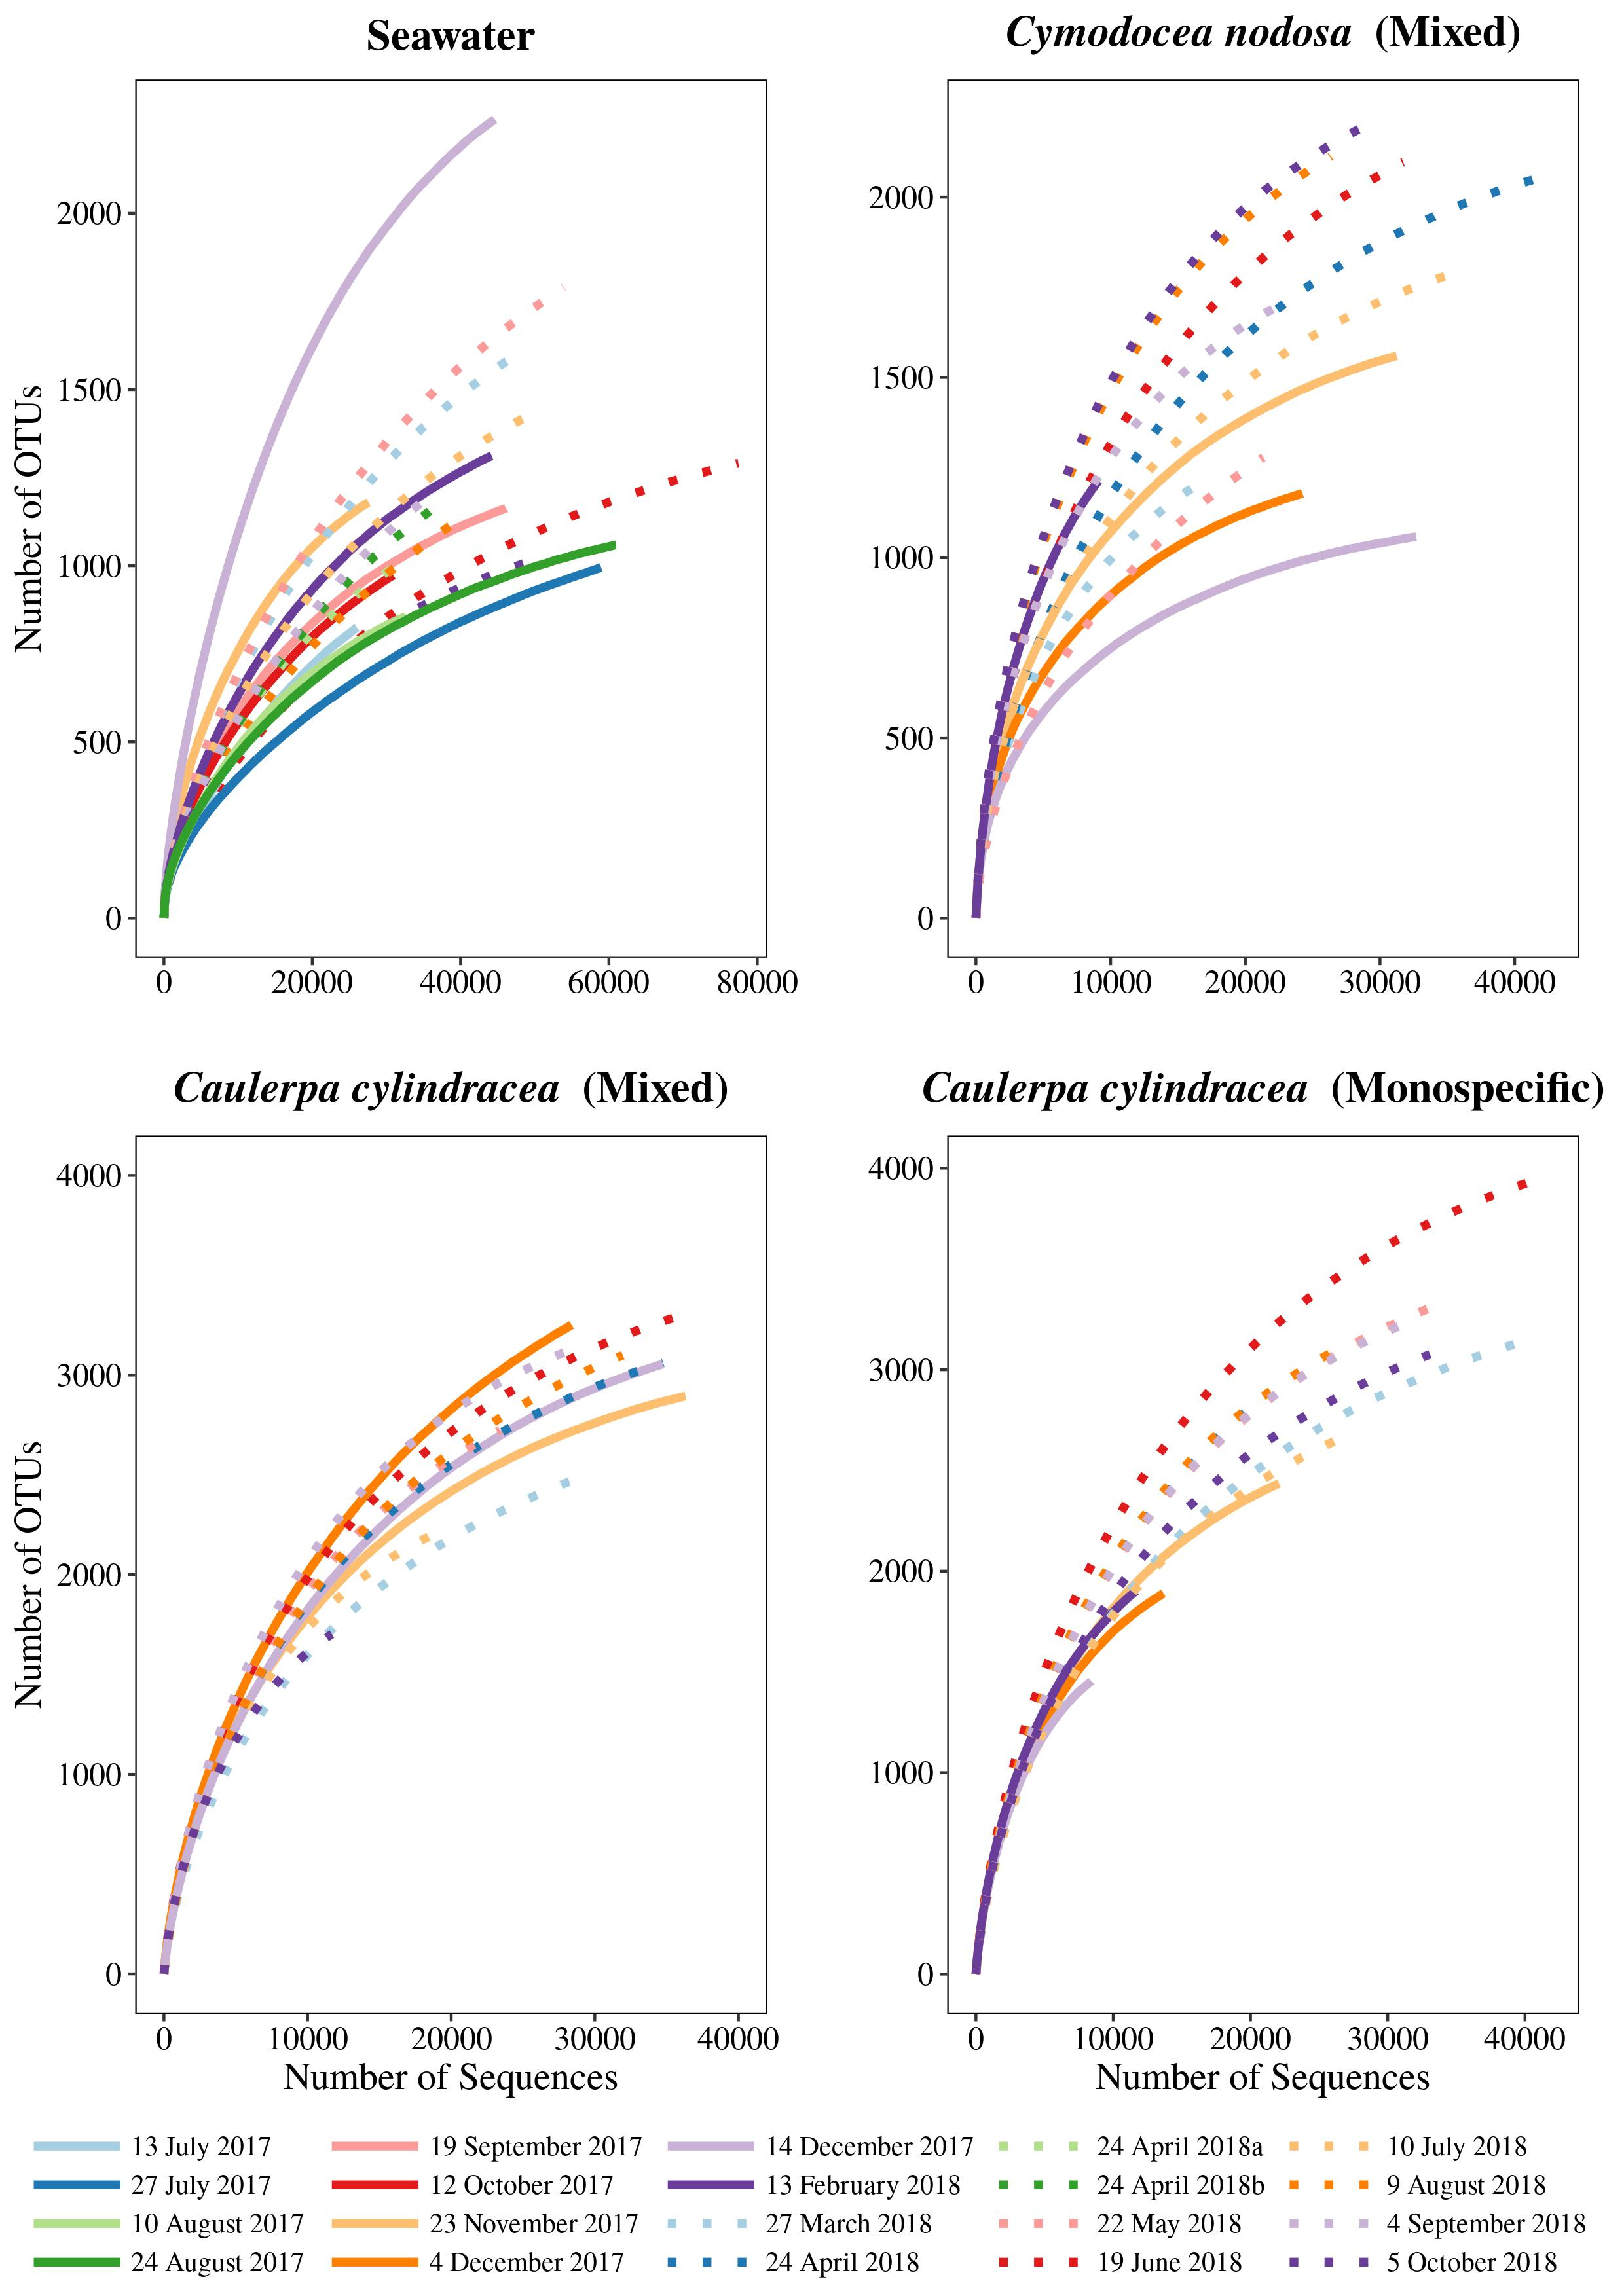
\includegraphics[width=0.85\linewidth]{/home/marino/Work/repositories/Korlevic_EpiphyticDynamics_FrontMicrobiol_2021/results/figures/rarefaction} 

}

\caption{Rarefaction curves of bacterial and archaeal communities from the surfaces of the macrophytes \textit{C. nodosa} (mixed settlement) and \textit{C. cylindracea} (mixed and monospecific settlement) and in the ambient seawater.\label{rarefaction}}\label{fig:unnamed-chunk-1}
\end{figure}

\begin{figure}[H]

{\centering 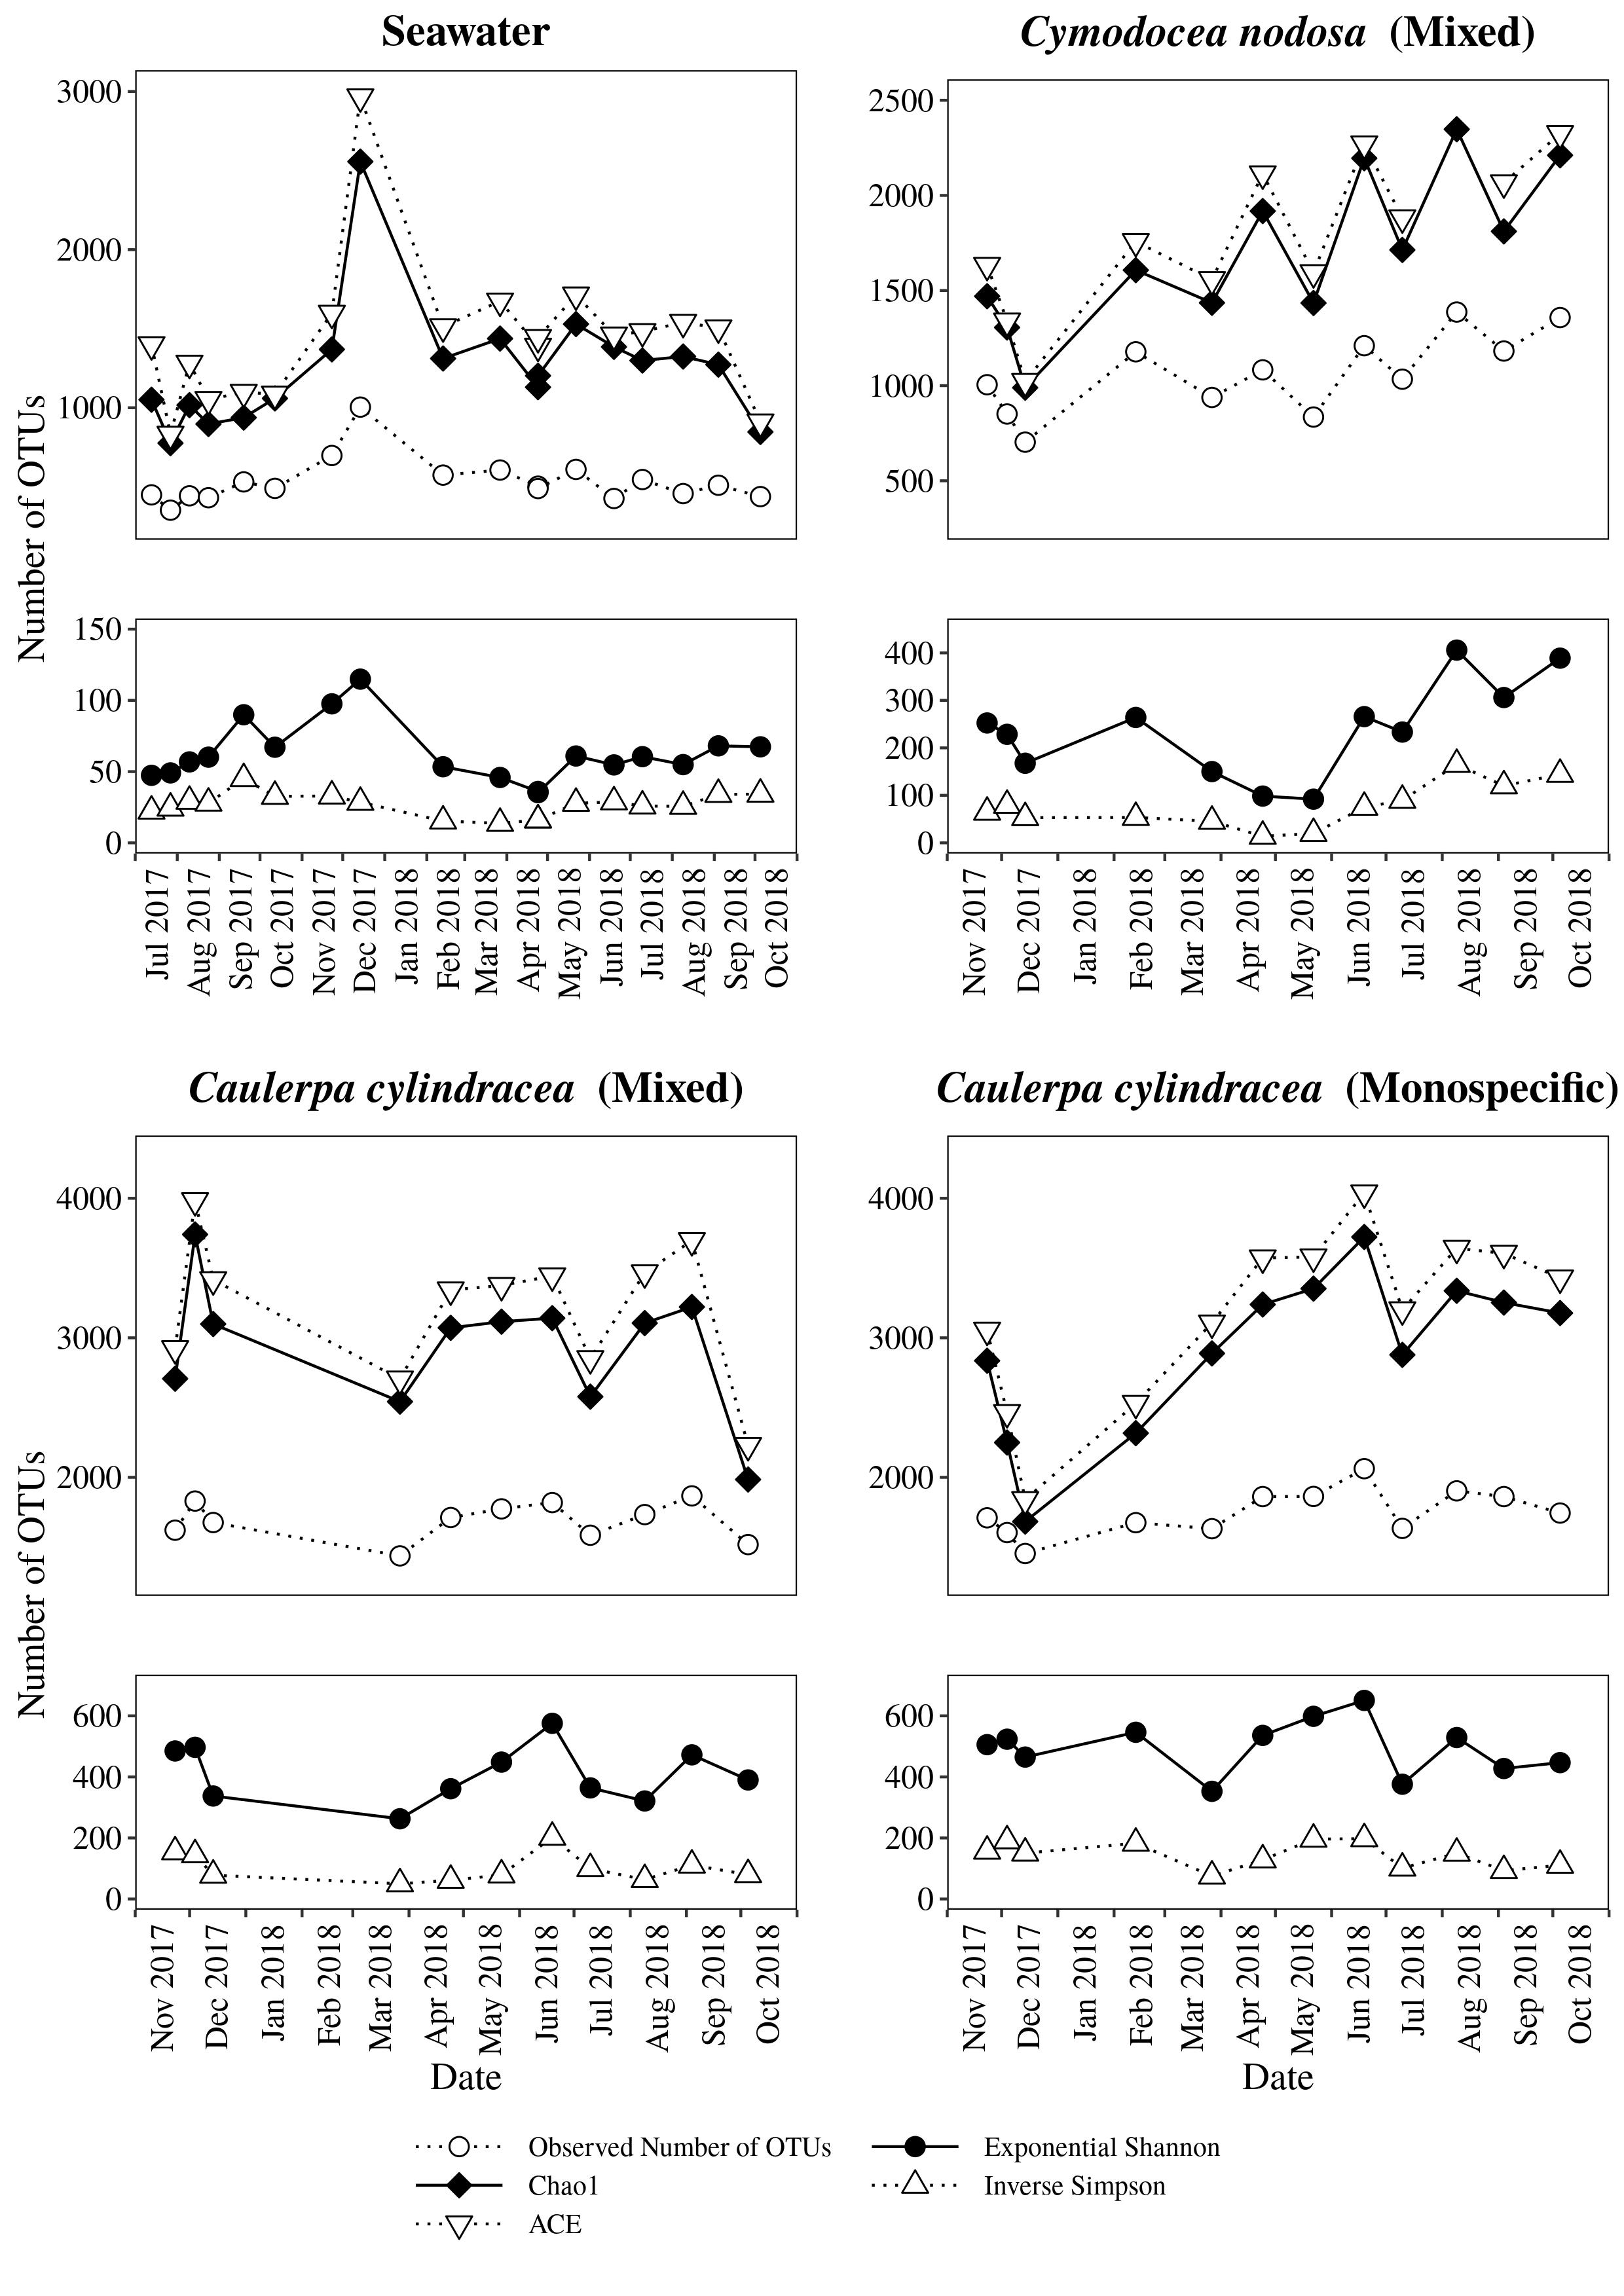
\includegraphics[width=0.85\linewidth]{/home/marino/Work/repositories/Korlevic_EpiphyticDynamics_FrontMicrobiol_2021/results/figures/calculators} 

}

\caption{Seasonal dynamics of observed number of OTUs, Chao1, ACE, exponential of the Shannon diversity index and Inverse Simpson index of bacterial and archaeal communities from the surfaces of the macrophytes \textit{C. nodosa} (mixed settlement) and \textit{C. cylindracea} (mixed and monospecific settlement) and in the ambient seawater.\label{calculators}}\label{fig:unnamed-chunk-2}
\end{figure}

\begin{figure}[H]

{\centering \includegraphics[width=0.85\linewidth]{/home/marino/Work/repositories/Korlevic_EpiphyticDynamics_FrontMicrobiol_2021/results/figures/chloroplast_bar_plot} 

}

\caption{Relative contribution of chloroplast sequences on the surfaces of the macrophytes \textit{C. nodosa} (mixed settlement) and \textit{C. cylindracea} (mixed and monospecific settlement) and in the ambient seawater.\label{chloroplast}}\label{fig:unnamed-chunk-3}
\end{figure}

\hypertarget{supplementary-table}{%
\subsection{Supplementary table}\label{supplementary-table}}

\begingroup\fontsize{9}{11}\selectfont

\begin{longtable}[t]{>{\centering\arraybackslash}p{6em}ccccc}
\caption{\label{tab:nseq_notus}Sample ID, community type, sampling date and season, no. of sequences and no. of OTUs of each sample. The number of sequences and OTUs was calculated after exclusion of sequences without known relatives (no relative sequences) and eukaryotic, chloroplast and mitochondrial sequences.\label{nseq_notus}}\\
\toprule
\textbf{Sample ID} & \textbf{Community Type} & \textbf{Date} & \textbf{Season} & \textbf{No. of Sequences} & \textbf{No. of OTUs}\\
\midrule
\endfirsthead
\caption[]{Sample ID, community type, sampling date and season, no. of sequences and no. of OTUs of each sample. The number of sequences and OTUs was calculated after exclusion of sequences without known relatives (no relative sequences) and eukaryotic, chloroplast and mitochondrial sequences.\label{nseq_notus} \textit{(continued)}}\\
\toprule
\textbf{Sample ID} & \textbf{Community Type} & \textbf{Date} & \textbf{Season} & \textbf{No. of Sequences} & \textbf{No. of OTUs}\\
\midrule
\endhead

\endfoot
\bottomrule
\endlastfoot
3 & Seawater & 13 July 2017 & Summer & 26,006 & 825\\
5 & Seawater & 27 July 2017 & Summer & 58,951 & 995\\
7 & Seawater & 10 August 2017 & Summer & 32,623 & 856\\
9 & Seawater & 24 August 2017 & Summer & 60,938 & 1,059\\
11 & Seawater & 19 September 2017 & Summer & 46,106 & 1,163\\
13 & Seawater & 12 October 2017 & Autumn & 30,905 & 973\\
15 & Seawater & 23 November 2017 & Autumn & 27,582 & 1,180\\
17 & Seawater & 14 December 2017 & Autumn & 44,591 & 2,267\\
19 & Seawater & 13 February 2018 & Winter & 44,193 & 1,312\\
21 & Seawater & 27 March 2018 & Winter & 46,352 & 1,583\\
23a & Seawater & 24 April 2018 & Spring & 30,976 & 995\\
23b & Seawater & 24 April 2018 & Spring & 38,565 & 1,196\\
25 & Seawater & 22 May 2018 & Spring & 53,872 & 1,791\\
27 & Seawater & 19 June 2018 & Spring & 77,463 & 1,291\\
29 & Seawater & 10 July 2018 & Summer & 50,786 & 1,443\\
31 & Seawater & 9 August 2018 & Summer & 39,039 & 1,120\\
33 & Seawater & 4 September 2018 & Summer & 36,201 & 1,205\\
35 & Seawater & 5 October 2018 & Autumn & 49,585 & 1,014\\
37 & \textit{Cymodocea nodosa} (Mixed) & 23 November 2017 & Autumn & 31,241 & 1,560\\
41 & \textit{Cymodocea nodosa} (Mixed) & 4 December 2017 & Autumn & 24,241 & 1,178\\
45 & \textit{Cymodocea nodosa} (Mixed) & 14 December 2017 & Autumn & 32,686 & 1,058\\
49 & \textit{Cymodocea nodosa} (Mixed) & 13 February 2018 & Winter & 9,091 & 1,213\\
52 & \textit{Cymodocea nodosa} (Mixed) & 27 March 2018 & Winter & 17,000 & 1,215\\
55 & \textit{Cymodocea nodosa} (Mixed) & 24 April 2018 & Spring & 42,653 & 2,063\\
58 & \textit{Cymodocea nodosa} (Mixed) & 22 May 2018 & Spring & 21,337 & 1,278\\
61 & \textit{Cymodocea nodosa} (Mixed) & 19 June 2018 & Spring & 31,726 & 2,097\\
64 & \textit{Cymodocea nodosa} (Mixed) & 10 July 2018 & Summer & 35,746 & 1,793\\
67 & \textit{Cymodocea nodosa} (Mixed) & 9 August 2018 & Summer & 26,360 & 2,113\\
70 & \textit{Cymodocea nodosa} (Mixed) & 4 September 2018 & Summer & 23,276 & 1,713\\
73 & \textit{Cymodocea nodosa} (Mixed) & 5 October 2018 & Autumn & 29,910 & 2,216\\
38 & \textit{Caulerpa cylindracea} (Mixed) & 23 November 2017 & Autumn & 36,318 & 2,895\\
42 & \textit{Caulerpa cylindracea} (Mixed) & 4 December 2017 & Autumn & 28,388 & 3,251\\
46 & \textit{Caulerpa cylindracea} (Mixed) & 14 December 2017 & Autumn & 34,721 & 3,055\\
53 & \textit{Caulerpa cylindracea} (Mixed) & 27 March 2018 & Winter & 28,688 & 2,478\\
56 & \textit{Caulerpa cylindracea} (Mixed) & 24 April 2018 & Spring & 34,765 & 3,060\\
59 & \textit{Caulerpa cylindracea} (Mixed) & 22 May 2018 & Spring & 23,403 & 2,723\\
62 & \textit{Caulerpa cylindracea} (Mixed) & 19 June 2018 & Spring & 36,487 & 3,310\\
65 & \textit{Caulerpa cylindracea} (Mixed) & 10 July 2018 & Summer & 18,486 & 2,192\\
68 & \textit{Caulerpa cylindracea} (Mixed) & 9 August 2018 & Summer & 31,953 & 3,099\\
71 & \textit{Caulerpa cylindracea} (Mixed) & 4 September 2018 & Summer & 29,280 & 3,152\\
74 & \textit{Caulerpa cylindracea} (Mixed) & 5 October 2018 & Autumn & 11,698 & 1,702\\
39 & \textit{Caulerpa cylindracea} (Monospecific) & 23 November 2017 & Autumn & 22,086 & 2,435\\
43 & \textit{Caulerpa cylindracea} (Monospecific) & 4 December 2017 & Autumn & 13,661 & 1,890\\
47 & \textit{Caulerpa cylindracea} (Monospecific) & 14 December 2017 & Autumn & 8,408 & 1,454\\
51 & \textit{Caulerpa cylindracea} (Monospecific) & 13 February 2018 & Winter & 11,673 & 1,902\\
54 & \textit{Caulerpa cylindracea} (Monospecific) & 27 March 2018 & Winter & 39,469 & 3,131\\
57 & \textit{Caulerpa cylindracea} (Monospecific) & 24 April 2018 & Spring & 20,299 & 2,832\\
60 & \textit{Caulerpa cylindracea} (Monospecific) & 22 May 2018 & Spring & 33,042 & 3,305\\
63 & \textit{Caulerpa cylindracea} (Monospecific) & 19 June 2018 & Spring & 41,852 & 3,964\\
66 & \textit{Caulerpa cylindracea} (Monospecific) & 10 July 2018 & Summer & 27,036 & 2,673\\
69 & \textit{Caulerpa cylindracea} (Monospecific) & 9 August 2018 & Summer & 26,736 & 3,114\\
72 & \textit{Caulerpa cylindracea} (Monospecific) & 4 September 2018 & Summer & 31,872 & 3,246\\
75 & \textit{Caulerpa cylindracea} (Monospecific) & 5 October 2018 & Autumn & 33,086 & 3,076\\*
\end{longtable}
\endgroup{}

\begingroup\fontsize{9}{11}\selectfont

\begin{longtable}[t]{>{\centering\arraybackslash}m{10em}>{\centering\arraybackslash}m{10em}cc>{\centering\arraybackslash}m{6em}>{\centering\arraybackslash}m{6em}}
\caption{\label{tab:calculators}Richness estimators and diversity indices of each community type. Calculations were done after normalization to the minimum number of reads per sample.\label{calculators_community_type}}\\
\toprule
\textbf{Community Type} & \textbf{Observed No. of OTUs} & \textbf{Chao1} & \textbf{ACE} & \textbf{Exponential Shannon} & \textbf{Inverse Simpson}\\
\midrule
\endfirsthead
\caption[]{Richness estimators and diversity indices of each community type. Calculations were done after normalization to the minimum number of reads per sample.\label{calculators_community_type} \textit{(continued)}}\\
\toprule
\textbf{Community Type} & \textbf{Observed No. of OTUs} & \textbf{Chao1} & \textbf{ACE} & \textbf{Exponential Shannon} & \textbf{Inverse Simpson}\\
\midrule
\endhead

\endfoot
\bottomrule
\endlastfoot
Seawater & 531.0  ±  143.9 & 1,244.5  ±  392.7 & 1,441.1  ±  458.7 & 62.2  ±   20.5 & 26.7  ±   8.0\\
\textit{Cymodocea nodosa} (Mixed) & 1,063.7  ±  210.6 & 1,703.2  ±  409.9 & 1,838.8  ±  437.3 & 237.8  ±  100.4 & 76.9  ±  46.6\\
\textit{Caulerpa cylindracea} (Mixed) & 1,688.4  ±  136.6 & 2,936.9  ±  460.2 & 3,220.7  ±  497.2 & 410.4  ±   92.5 & 102.2  ±  47.2\\
\textit{Caulerpa cylindracea} (Monospecific) & 1,750.4  ±  165.7 & 2,911.0  ±  575.0 & 3,171.7  ±  622.1 & 496.4  ±   87.1 & 144.4  ±  42.6\\*
\end{longtable}
\endgroup{}

\newpage

\begingroup\fontsize{9}{11}\selectfont

\begin{longtable}[t]{>{\centering\arraybackslash}m{6em}ccccc}
\caption{\label{tab:calculator_statistics}Statistic of richness estimator and diversity index parameters for different community types. Parameters were tested by applying the Kruskal-Wallis \textit{H} test followed by a pairwise comparison using the Mann-Whitney \textit{U} test. Bonferroni correction was used to address the problem of multiple comparisons.\label{calculator_statistics}}\\
\toprule
\multicolumn{1}{c}{\textbf{ }} & \multicolumn{3}{c}{\textbf{Kruskal-Wallis \textit{H} test}} & \multicolumn{2}{c}{\textbf{Mann-Whitney \textit{U} test}} \\
\cmidrule(l{3pt}r{3pt}){2-4} \cmidrule(l{3pt}r{3pt}){5-6}
\textbf{Parameter} & \textbf{\textit{H}} & \textbf{\textit{df}} & \textbf{\textit{p}} & \textbf{Comparisons Between Community Types} & \textbf{\textit{p}}\\
\midrule
\endfirsthead
\caption[]{Statistic of richness estimator and diversity index parameters for different community types. Parameters were tested by applying the Kruskal-Wallis \textit{H} test followed by a pairwise comparison using the Mann-Whitney \textit{U} test. Bonferroni correction was used to address the problem of multiple comparisons.\label{calculator_statistics} \textit{(continued)}}\\
\toprule
\multicolumn{1}{c}{\textbf{ }} & \multicolumn{3}{c}{\textbf{Kruskal-Wallis \textit{H} test}} & \multicolumn{2}{c}{\textbf{Mann-Whitney \textit{U} test}} \\
\cmidrule(l{3pt}r{3pt}){2-4} \cmidrule(l{3pt}r{3pt}){5-6}
\textbf{Parameter} & \textbf{\textit{H}} & \textbf{\textit{df}} & \textbf{\textit{p}} & \textbf{Comparisons Between Community Types} & \textbf{\textit{p}}\\
\midrule
\endhead

\endfoot
\bottomrule
\endlastfoot
 &  &  &  & Seawater – \textit{Cymodocea nodosa} (Mixed) & < 0.0001\\
\nopagebreak
 &  &  &  & Seawater – \textit{Caulerpa cylindracea} (Mixed) & < 0.0001\\
\nopagebreak
 &  &  &  & Seawater – \textit{Caulerpa cylindracea} (Monospecific) & < 0.0001\\
\nopagebreak
 &  &  &  & \textit{Cymodocea nodosa} (Mixed) – \textit{Caulerpa cylindracea} (Mixed) & < 0.001\\
\nopagebreak
 &  &  &  & \textit{Cymodocea nodosa} (Mixed) – \textit{Caulerpa cylindracea} (Monospecific) & < 0.001\\
\nopagebreak
\multirow{-6}{6em}{\centering\arraybackslash Observed No. of OTUs} & \multirow{-6}{*}{\centering\arraybackslash 44.8} & \multirow{-6}{*}{\centering\arraybackslash 3} & \multirow{-6}{*}{\centering\arraybackslash < 0.0001} & \textit{Caulerpa cylindracea} (Mixed) – \textit{Caulerpa cylindracea} (Monospecific) & 1.00\\
\cmidrule{1-6}\pagebreak[0]
 &  &  &  & Seawater – \textit{Cymodocea nodosa} (Mixed) & < 0.01\\
\nopagebreak
 &  &  &  & Seawater – \textit{Caulerpa cylindracea} (Mixed) & < 0.0001\\
\nopagebreak
 &  &  &  & Seawater – \textit{Caulerpa cylindracea} (Monospecific) & < 0.0001\\
\nopagebreak
 &  &  &  & \textit{Cymodocea nodosa} (Mixed) – \textit{Caulerpa cylindracea} (Mixed) & < 0.0001\\
\nopagebreak
 &  &  &  & \textit{Cymodocea nodosa} (Mixed) – \textit{Caulerpa cylindracea} (Monospecific) & < 0.001\\
\nopagebreak
\multirow{-6}{6em}{\centering\arraybackslash Chao1} & \multirow{-6}{*}{\centering\arraybackslash 38.3} & \multirow{-6}{*}{\centering\arraybackslash 3} & \multirow{-6}{*}{\centering\arraybackslash < 0.0001} & \textit{Caulerpa cylindracea} (Mixed) – \textit{Caulerpa cylindracea} (Monospecific) & 1.00\\
\cmidrule{1-6}\pagebreak[0]
 &  &  &  & Seawater – \textit{Cymodocea nodosa} (Mixed) & < 0.05\\
\nopagebreak
 &  &  &  & Seawater – \textit{Caulerpa cylindracea} (Mixed) & < 0.0001\\
\nopagebreak
 &  &  &  & Seawater – \textit{Caulerpa cylindracea} (Monospecific) & < 0.0001\\
\nopagebreak
 &  &  &  & \textit{Cymodocea nodosa} (Mixed) – \textit{Caulerpa cylindracea} (Mixed) & < 0.0001\\
\nopagebreak
 &  &  &  & \textit{Cymodocea nodosa} (Mixed) – \textit{Caulerpa cylindracea} (Monospecific) & < 0.001\\
\nopagebreak
\multirow{-6}{6em}{\centering\arraybackslash ACE} & \multirow{-6}{*}{\centering\arraybackslash 37.1} & \multirow{-6}{*}{\centering\arraybackslash 3} & \multirow{-6}{*}{\centering\arraybackslash < 0.0001} & \textit{Caulerpa cylindracea} (Mixed) – \textit{Caulerpa cylindracea} (Monospecific) & 1.00\\
\cmidrule{1-6}\pagebreak[0]
 &  &  &  & Seawater – \textit{Cymodocea nodosa} (Mixed) & < 0.0001\\
\nopagebreak
 &  &  &  & Seawater – \textit{Caulerpa cylindracea} (Mixed) & < 0.0001\\
\nopagebreak
 &  &  &  & Seawater – \textit{Caulerpa cylindracea} (Monospecific) & < 0.0001\\
\nopagebreak
 &  &  &  & \textit{Cymodocea nodosa} (Mixed) – \textit{Caulerpa cylindracea} (Mixed) & < 0.01\\
\nopagebreak
 &  &  &  & \textit{Cymodocea nodosa} (Mixed) – \textit{Caulerpa cylindracea} (Monospecific) & < 0.0001\\
\nopagebreak
\multirow{-6}{6em}{\centering\arraybackslash Exponential Shannon} & \multirow{-6}{*}{\centering\arraybackslash 43.3} & \multirow{-6}{*}{\centering\arraybackslash 3} & \multirow{-6}{*}{\centering\arraybackslash < 0.0001} & \textit{Caulerpa cylindracea} (Mixed) – \textit{Caulerpa cylindracea} (Monospecific) & 0.26\\
\cmidrule{1-6}\pagebreak[0]
 &  &  &  & Seawater – \textit{Cymodocea nodosa} (Mixed) & < 0.01\\
\nopagebreak
 &  &  &  & Seawater – \textit{Caulerpa cylindracea} (Mixed) & < 0.0001\\
\nopagebreak
 &  &  &  & Seawater – \textit{Caulerpa cylindracea} (Monospecific) & < 0.0001\\
\nopagebreak
 &  &  &  & \textit{Cymodocea nodosa} (Mixed) – \textit{Caulerpa cylindracea} (Mixed) & 1.00\\
\nopagebreak
 &  &  &  & \textit{Cymodocea nodosa} (Mixed) – \textit{Caulerpa cylindracea} (Monospecific) & < 0.01\\
\nopagebreak
\multirow{-6}{6em}{\centering\arraybackslash Inverse Simpson} & \multirow{-6}{*}{\centering\arraybackslash 34.8} & \multirow{-6}{*}{\centering\arraybackslash 3} & \multirow{-6}{*}{\centering\arraybackslash < 0.0001} & \textit{Caulerpa cylindracea} (Mixed) – \textit{Caulerpa cylindracea} (Monospecific) & 0.26\\*
\end{longtable}
\endgroup{}

\newpage
\blandscape
\begingroup\fontsize{9}{11}\selectfont

\begin{longtable}[t]{>{\centering\arraybackslash}m{8em}ccl}
\caption{\label{tab:core_otus_taxonomy_table}Taxonomic classification of OTUs present at every sampling date in each community type. Only ten OTUs with the highest number of sequences after normalization to the minimum number of reads per sample are shown. NR -- No Relative (sequences without known relatives within the corresponding group)\label{core_otus_taxonomy_table}}\\
\toprule
\textbf{Community Type} & \textbf{OTU Number} & \textbf{No. of Sequences} & \textbf{OTU Taxonomy}\\
\midrule
\endfirsthead
\caption[]{Taxonomic classification of OTUs present at every sampling date in each community type. Only ten OTUs with the highest number of sequences after normalization to the minimum number of reads per sample are shown. NR -- No Relative (sequences without known relatives within the corresponding group)\label{core_otus_taxonomy_table} \textit{(continued)}}\\
\toprule
\textbf{Community Type} & \textbf{OTU Number} & \textbf{No. of Sequences} & \textbf{OTU Taxonomy}\\
\midrule
\endhead

\endfoot
\bottomrule
\endlastfoot
 & Otu00014 & 5092 & \textit{Bacteria}; \textit{Proteobacteria}; \textit{Alphaproteobacteria}; \textit{Rhodobacterales}; \textit{Rhodobacteraceae}; \textit{Rhodobacteraceae} (NR)\\
\nopagebreak
 & Otu00020 & 3188 & \textit{Bacteria}; \textit{Proteobacteria}; \textit{Alphaproteobacteria}; \textit{Rhodobacterales}; \textit{Rhodobacteraceae}; \textit{Rhodobacteraceae} (NR)\\
\nopagebreak
 & Otu00019 & 3026 & \textit{Bacteria}; \textit{Cyanobacteria}; \textit{Cyanobacteriia}; \textit{Cyanobacteriales}; \textit{Xenococcaceae}; \textit{Pleurocapsa}\\
\nopagebreak
 & Otu00030 & 2014 & \textit{Bacteria}; \textit{Proteobacteria}; \textit{Alphaproteobacteria}; \textit{Rhodobacterales}; \textit{Rhodobacteraceae}; \textit{Rhodobacteraceae} (NR)\\
\nopagebreak
 & Otu00013 & 1884 & \textit{Bacteria}; \textit{Proteobacteria}; \textit{Alphaproteobacteria}; \textit{Rhodobacterales}; \textit{Rhodobacteraceae}; \textit{Rhodobacteraceae} (NR)\\
\nopagebreak
 & Otu00032 & 1586 & \textit{Bacteria}; \textit{Verrucomicrobiota}; \textit{Verrucomicrobiae}; \textit{Opitutales}; \textit{Puniceicoccaceae}; \textit{Lentimonas}\\
\nopagebreak
 & Otu00059 & 1469 & \textit{Bacteria}; \textit{Proteobacteria}; \textit{Gammaproteobacteria}; \textit{Burkholderiales}; \textit{Methylophilaceae}; \textit{Methylotenera}\\
\nopagebreak
 & Otu00005 & 1337 & \textit{Bacteria}; \textit{Proteobacteria}; \textit{Alphaproteobacteria}; \textit{Rhodobacterales}; \textit{Rhodobacteraceae}; \textit{Rhodobacteraceae} (NR)\\
\nopagebreak
 & Otu00050 & 1264 & \textit{Bacteria}; \textit{Proteobacteria}; \textit{Alphaproteobacteria}; \textit{Rhodobacterales}; \textit{Rhodobacteraceae}; \textit{Rhodobacteraceae} (NR)\\
\nopagebreak
\multirow{-10}{8em}{\centering\arraybackslash \textit{Cymodocea nodosa} (Mixed)} & Otu00029 & 1162 & \textit{Bacteria}; \textit{Proteobacteria}; \textit{Alphaproteobacteria}; \textit{Rhodobacterales}; \textit{Rhodobacteraceae}; \textit{Rhodobacteraceae} (NR)\\
\cmidrule{1-4}\pagebreak[0]
 & Otu00011 & 4051 & \textit{Bacteria}; \textit{Desulfobacterota}; \textit{Desulfobacteria}; \textit{Desulfobacterales}; \textit{Desulfosarcinaceae}; \textit{Desulfatitalea}\\
\nopagebreak
 & Otu00010 & 3436 & \textit{Bacteria}; \textit{Desulfobacterota}; \textit{Desulfobulbia}; \textit{Desulfobulbales}; \textit{Desulfocapsaceae}; \textit{Desulfocapsaceae} (NR)\\
\nopagebreak
 & Otu00013 & 2531 & \textit{Bacteria}; \textit{Proteobacteria}; \textit{Alphaproteobacteria}; \textit{Rhodobacterales}; \textit{Rhodobacteraceae}; \textit{Rhodobacteraceae} (NR)\\
\nopagebreak
 & Otu00021 & 1859 & \textit{Bacteria}; \textit{Desulfobacterota}; \textit{Desulfobulbia}; \textit{Desulfobulbales}; \textit{Desulfocapsaceae}; \textit{Desulfocapsaceae} (NR)\\
\nopagebreak
 & Otu00025 & 1481 & \textit{Bacteria}; \textit{Desulfobacterota}; \textit{Desulfobulbia}; \textit{Desulfobulbales}; \textit{Desulfocapsaceae}; SEEP-SRB4\\
\nopagebreak
 & Otu00037 & 1209 & \textit{Bacteria}; \textit{Desulfobacterota}; \textit{Desulfobulbia}; \textit{Desulfobulbales}; \textit{Desulfobulbaceae}; \textit{Desulfobulbus}\\
\nopagebreak
 & Otu00033 & 1189 & \textit{Bacteria}; \textit{Desulfobacterota}; \textit{Desulfobulbia}; \textit{Desulfobulbales}; \textit{Desulfocapsaceae}; \textit{Desulfocapsaceae} (NR)\\
\nopagebreak
 & Otu00044 & 1042 & \textit{Bacteria}; \textit{Desulfobacterota}; \textit{Desulfobulbia}; \textit{Desulfobulbales}; \textit{Desulfocapsaceae}; \textit{Desulfocapsaceae} (NR)\\
\nopagebreak
 & Otu00019 & 1012 & \textit{Bacteria}; \textit{Cyanobacteria}; \textit{Cyanobacteriia}; \textit{Cyanobacteriales}; \textit{Xenococcaceae}; \textit{Pleurocapsa}\\
\nopagebreak
\multirow{-10}{8em}{\centering\arraybackslash \textit{Caulerpa cylindracea} (Mixed)} & Otu00046 & 982 & \textit{Bacteria}; \textit{Desulfobacterota}; \textit{Desulfobulbia}; \textit{Desulfobulbales}; \textit{Desulfocapsaceae}; \textit{Desulfotalea}\\
\cmidrule{1-4}\pagebreak[0]
 & Otu00010 & 3572 & \textit{Bacteria}; \textit{Desulfobacterota}; \textit{Desulfobulbia}; \textit{Desulfobulbales}; \textit{Desulfocapsaceae}; \textit{Desulfocapsaceae} (NR)\\
\nopagebreak
 & Otu00011 & 2977 & \textit{Bacteria}; \textit{Desulfobacterota}; \textit{Desulfobacteria}; \textit{Desulfobacterales}; \textit{Desulfosarcinaceae}; \textit{Desulfatitalea}\\
\nopagebreak
 & Otu00013 & 2109 & \textit{Bacteria}; \textit{Proteobacteria}; \textit{Alphaproteobacteria}; \textit{Rhodobacterales}; \textit{Rhodobacteraceae}; \textit{Rhodobacteraceae} (NR)\\
\nopagebreak
 & Otu00021 & 1931 & \textit{Bacteria}; \textit{Desulfobacterota}; \textit{Desulfobulbia}; \textit{Desulfobulbales}; \textit{Desulfocapsaceae}; \textit{Desulfocapsaceae} (NR)\\
\nopagebreak
 & Otu00025 & 1912 & \textit{Bacteria}; \textit{Desulfobacterota}; \textit{Desulfobulbia}; \textit{Desulfobulbales}; \textit{Desulfocapsaceae}; SEEP-SRB4\\
\nopagebreak
 & Otu00033 & 1613 & \textit{Bacteria}; \textit{Desulfobacterota}; \textit{Desulfobulbia}; \textit{Desulfobulbales}; \textit{Desulfocapsaceae}; \textit{Desulfocapsaceae} (NR)\\
\nopagebreak
 & Otu00040 & 1289 & \textit{Bacteria}; \textit{Desulfobacterota}; \textit{Desulfobacteria}; \textit{Desulfobacterales}; \textit{Desulfobacteraceae}; \textit{Desulfobacteraceae} (NR)\\
\nopagebreak
 & Otu00046 & 1089 & \textit{Bacteria}; \textit{Desulfobacterota}; \textit{Desulfobulbia}; \textit{Desulfobulbales}; \textit{Desulfocapsaceae}; \textit{Desulfotalea}\\
\nopagebreak
 & Otu00037 & 1058 & \textit{Bacteria}; \textit{Desulfobacterota}; \textit{Desulfobulbia}; \textit{Desulfobulbales}; \textit{Desulfobulbaceae}; \textit{Desulfobulbus}\\
\nopagebreak
\multirow{-10}{8em}{\centering\arraybackslash \textit{Caulerpa cylindracea} (Monospecific)} & Otu00058 & 950 & \textit{Bacteria}; \textit{Desulfobacterota}; \textit{Desulfobacteria}; \textit{Desulfobacterales}; \textit{Desulfosarcinaceae}; \textit{Desulfatitalea}\\*
\end{longtable}
\endgroup{}
\elandscape

\end{document}
